\documentclass[12pt,letterpaper]{article}

%Packages
\usepackage{fixltx2e}
\usepackage{textcomp}
\usepackage{fullpage}
\usepackage{natbib}
\usepackage{float}
\usepackage{latexsym}
\usepackage{hyperref}
\usepackage{url}
%\usepackage{html}
\usepackage{hyperref}
\usepackage{epsfig}
\usepackage{graphicx}
\usepackage{amssymb}
\usepackage{amsmath}
\usepackage{bm}
\usepackage{array}
\usepackage[version=3]{mhchem}
\usepackage{ifthen}
\usepackage{caption}
\usepackage{hyperref}
\usepackage{amsthm}
\usepackage{amstext}
\usepackage{enumerate}
\usepackage[osf]{mathpazo}
\pagenumbering{arabic}

%Pagination style and stuff
\linespread{1.66}
\raggedright
\setlength{\parindent}{0.5in}
\setcounter{secnumdepth}{0} 
\renewcommand{\section}[1]{%
\bigskip
\begin{center}
\begin{Large}
\normalfont\scshape #1
\medskip
\end{Large}
\end{center}}
\renewcommand{\subsection}[1]{%
\bigskip
\begin{center}
\begin{large}
\normalfont\itshape #1
\end{large}
\end{center}}
\renewcommand{\subsubsection}[1]{%
\vspace{2ex}
\noindent
\textit{#1.}---}
\renewcommand{\tableofcontents}{}
\bibpunct{(}{)}{;}{a}{}{,}

%---------------------------------------------
%
%       START
%
%---------------------------------------------

\begin{document}
%\modulolinenumbers[1]     % Line numbering on every line

%Running head
\begin{flushright}
Version dated: \today
\end{flushright}
\bigskip
\noindent RH: Missing data and topology in total evidence approach

\bigskip
\medskip
\begin{center}

\noindent{\Large \bf Effect of missing data on topological inference using a total evidence approach}
%Or do we put results in the title: Bayesian analysis and increased sampling of living taxa improves topological inference when using a total evidence approach
\bigskip

%Authors
\noindent {\normalsize \sc Thomas Guillerme$^1$$^,$$^2$, and Natalie Cooper$^1$$^,$$^2$}\\
\noindent {\small \it 
$^1$School of Natural Sciences, Trinity College Dublin, Dublin 2, Ireland;\\
$^2$Trinity Centre for Biodiversity Research, Trinity College Dublin, Dublin 2, Ireland;}\\
\end{center}
\medskip
\noindent{\bf Corresponding author:} Thomas Guillerme, School of Natural Sciences, Trinity College Dublin, Dublin 2, Ireland; E-mail: guillert@tcd.ie; Fax: +353 1 6778094; Tel: +353 1 896 2571.\\
\vspace{1in}

%---------------------------------------------
%
%       ABSTRACT
%
%---------------------------------------------

\newpage
\begin{abstract}
Living species represent a marginal part of all species that have ever lived. Ignoring fossil taxa may lead to misinterpretation of macroevolutionary patterns and processes such as trends in species richness, biogeographical history or paleoecology. This fact has led to an increasing consensus among scientists that both living and fossil taxa must be included in macroevolutionary studies. One approach called Total Evidence, uses molecular data from living taxa and morphological data from both living and fossil taxa to infer phylogenies with both living and fossil taxa at the tips. Although the Total Evidence approach seems very promising, it requires a lot of data and is therefore likely to suffer from missing data issues which may affect its ability to infer correct phylogenies.

In this study we assess the effect of missing data on tree topologies inferred from Total Evidence matrices. Using simulations we investigate three major factors that directly affect the completeness of the morphological part of the matrix: (1) the proportion of living taxa with no morphological data, (2) the amount of missing data in the fossil record, and (3) the overall number of morphological characters in the matrix. 

We find that, when using a clade conservative metric such as Robinson-Foulds distance, Bayesian consensus trees recovers the right topology better than Maximum Likelihood or than a subset of Bayesian posterior tree distributions and this regardless of the amount of missing data (minimal tree similarity of 0.69 in the worst scenario). Regarding the data, good topological recovery is not related to the amount of missing data \textit{per se} but to the amount of data overlap. The two factors that influences the most this data overlap are the parameters 1 (proportion of coded living taxa) and 3 (number of morphological characters).
\end{abstract}

\noindent (Keywords: missing data, Total Evidence, Bayesian, Maximum Likelihood, topology)\\

\vspace{1.5in}

\newpage 

%---------------------------------------------
%
%       INTRODUCTION
%
%---------------------------------------------

\section{Introduction}

Although most species that have ever lived are now extinct \citep{novacek1992ext,raup1993extinction}, the majority of macroevolutionary studies focus solely on living species \citep[e.g.][]{meredithimpacts2011,jetzthe2012}. Ignoring fossil taxa may lead to misinterpretation of macroevolutionary patterns and processes such as the timing of diversification events \citep[e.g.][]{pyrondivergence2011}, relationships among lineages \citep[e.g.][]{manosphylogeny2007} or niche occupancy \citep[e.g.][]{pearmanniche2008}. This has led to increasing consensus among scientists that fossil taxa must be included in macroevolutionary studies \citep{jacksonwhat2006,quentaldiversity2010,dietlconservation2011,slaterunifying2013,fritzdiversity2013}. However, to do this we need to be able to place living and fossil taxa into the same phylogenies; a task that remains difficult despite recent methodological developments \citep[e.g.][]{pyrondivergence2011,ronquista2012,schragocombining2013}. %Not a nice sentence

Up to now, three main approaches have been used to place both living and fossil taxa into phylogenies. These approaches differ mainly in whether they treat fossil taxa as tips or as nodes in the phylogeny, and in which part of the available fossil data is used (i.e. the age of the fossil only or both its age and morphology). Classical cladistic methods use matrices containing morphological data from both living and fossil taxa and treat each taxon as a tip in the phylogeny. Relationships among the taxa are then inferred using optimality criteria such as maximum parsimony \citep{simpson1945}. This approach is commonly used by paleontologists but it ignores the additional molecular data available from living species and does not allow use of probabilistic methods for dealing with phylogenetic uncertainty. Neontologists, on the other hand, more commonly use probabilistic approaches (e.g. Maximum Likelihood or Bayesian methods) based on matrices containing only molecular data from living species. Because fossil taxa do not usually have available DNA, fossils are used as nodes rather than tips in these phylogenies and their occurrence date are used to time calibrate phylogenies \citep{zuckerkandl1965}. There have been great improvements in the theory and application of these two approaches \citep[e.g.][]{bapsta2013,stadlerdating2013,heaththe2013} as well as much debate about the "best" approach to use \citep[e.g.][]{spencerefficacy2013,wrightbayesian2014}. However neither approach uses all the available data.

A final approach, known as the Total Evidence method, uses matrices containing molecular data from living taxa and morphological data from both living and fossil taxa \citep{eernissetaxonomic1993}. This approach treats every taxon as a tip in the phylogeny, uses the occurrence age of the fossils to time calibrate the phylogeny, and allows the use of probabilistic methods for estimating phylogenetic uncertainty \citep{ronquista2012}. Total Evidence methods have been successfully applied to empirical data \citep[e.g.][]{pyrondivergence2011,ronquista2012,schragocombining2013,slaterphylogenetic2013,beckancient2014}, and are becoming an increasingly popular way of adding fossil taxa to phylogenies. However, although the Total Evidence approach seems very promising, there is one big drawback in using this approach: it requires a lot of data that can be difficult (or impossible) to collect. The morphological data for living taxa is rarely collected when molecular data is available (e.g. \citealt{O'Leary08022013} \textit{vs.} \citealt{meredithimpacts2011}), and, for fossil taxa, the scarcity of the fossil record only allow to collect the data available (for example, in vertebrates, the hardest parts of the skeleton; \citealt{sansomfossilization2013}). Therefore Total Evidence matrices are likely to contain a lot of missing data that may affect the method's ability to infer correct topologies, branch lengths and support values \citep{salamin2003}. 

The effect of missing data on phylogenetic inferences has been widely studied \citep{wiensmissing2003,wiensmissing2006,wiensmissing2008,lemmonthe2009,rouresite-specific2011,sansomfossilization2013,pattinsonphylogeny2014,sansombias2014}. Missing molecular data has been seen by some authors as an issue because it can, in some part of the tree, decrease phylogenetic signal (i.e. the evolutionary information contained within the matrix allowing to infer topology and branch length), especially when using large matrices \citep{lemmonthe2009}. However, this may not be a major issue because phylogenetic signal is easily increased by: (i) including a "modest" number (~50) of highly-covered genes (i.e. a number of genes that are available for all taxa ; \citealt{rouresite-specific2011}); (ii) adding a greater number of taxa (especially slowly-evolving taxa or taxa close to the outgroup; \citealt{rouresite-specific2011}); and (iii) choosing more appropriate models of sequence evolution \citep{wiensmissing2006,wiensmissing2008,rouresite-specific2011}. Similarly, missing morphological data might be seen as either a major or minor issue for accurately inferring phylogenies depending on the study in question \citep{wiensmissing2003,sansomfossilization2013,pattinsonphylogeny2014}. Because soft-tissue characters are rarely preserved in the fossil record, missing data is mainly found in these characters, and is therefore not randomly distributed which can lead to biased placement of fossil taxa in phylogenies (e.g. \citealt{sansomfossilization2013} but see \citealt{pattinsonphylogeny2014}). However, the phylogenetic signal is not related to the amount of missing data \textit{per se} but to the number of informative characters for each taxon, therefore missing data is less of an issue than the number of shared informative characters \citep{kearneyfragmentary2002,wiensmissing2003,pattinsonphylogeny2014}.
% NC: I'm a little dubious of what this paragraph is trying to get at in places. We should discuss at some point. TG: my idea was to do the "literature-review" part of the intro: missing data is already widely studied (answer to the comment: "hun... We already knew that") but it has never been studied in TEM framework. And that's kind of the point we're getting toward with our work: we don't really care about the effect of missing data per se (i.e. what's the threshold were it starts fucking up the phylogeny) but more the fact that Bayesian fails.

Although missing data does not appear be a major problem in molecular and morphological matrices separately \citep{wiensmissing2003,wiensmissing2006,wiensmissing2008,rouresite-specific2011,pattinsonphylogeny2014}, it may become more of an issue in Total Evidence matrices containing both molecular and morphological data for living and fossil species. This may be particularly problematic as fossil taxa (generally) do not have molecular data, resulting in a large section of missing data. Until now, no attempt has been made to study the impact of this issue on phylogenetic inference from Total Evidence methods. % NC: Somewhere here you need to flag that you're only looking at topologies and briefly explain why.
In this study, we are interested in assessing the effect of missing data on the ability to recover a correct topology. Even though branch length is a second aspect of phylogenetic inferences equally important, topology is the first and most straightforward aspect reflecting phylogenetic signal (i.e. topological changes are discrete opposed to branch length changes are continuous). Also, interestingly, the effect of Total Evidence method has not been formally assessed in previous studies using fixed topology \citep{ronquista2012,schragocombining2013}.

Here we use a simulation approach to assess the effect of missing data on tree topologies inferred from Total Evidence matrices. Since the molecular part of a Total Evidence matrix acts like a "classical" molecular matrix containing only the living taxa \citep{ronquista2012}, the effect of missing data on such matrices is well known \citep{wiensmissing2006,wiensmissing2008,rouresite-specific2011}. Therefore, we focus only on missing data in the morphological part of the matrix. We investigate three major parameters that directly affect the completeness of the morphological part of the matrix:
\begin{enumerate}
\item the proportion of living taxa with no morphological data;
\item the proportion of missing data in the fossil taxa; and
\item the proportion of missing morphological characters for both living and fossil taxa in the matrix.
\end{enumerate} 
We remove data from a Total Evidence matrix by changing the values of these three parameters and then assess how this affects the topology of trees inferred using Maximum Likelihood and Bayesian methods. We chose these parameters because they reflect empirical biases in data availability. The advent of molecular phylogenetics means that morphological data for living species is rarely collected, and few people have the skills to identify characters needed for detailed phylogenetic analysis. Missing data in fossil taxa is very common due to preservation biases \citep{sansomfossilization2013}, and the overall number of characters depends on the effort of the people identifying them \citep[e.g.][]{O'Leary08022013}.

We find that the ability of recovering the correct topology can mainly be increased when using the Bayesian methods. Also minimizing the proportion of living taxa with no morphological data and the proportion of missing morphological characters improves the ability to recover the correct more than minimizing the proportion of missing data in the fossil record.

%---------------------------------------------
%
%       METHODS
%
%---------------------------------------------
 
\newpage

\section{Methods}
To explore how missing data in the morphological sections of Total Evidence matrices influences tree topology, we used the following protocol (note that we explain each step in detail below this general outline; Fig.~\ref{Fig_Outline}).
\begin{enumerate}
\item{Generating the matrix} \label{step:generate_matrix} \\
We randomly generated a birth-death tree (hereafter called the "true" tree) and used it to infer a matrix containing both molecular and morphological data for living and fossil taxa (hereafter called the "complete" matrix).
\item{Removing data} \label{step:remove_data} \\
We removed data from the morphological part of the "complete" matrix to simulate the effects of missing data by modifying three parameters (i) the proportion of living taxa with no morphological data ($M_{L}$), (ii) the proportion of missing data in the fossil taxa ($M_{F}$) and (iii) the proportion of missing morphological characters ($M_{C}$) (the resulting matrices are called hereafter "missing-data" matrices).
\item{Inferring phylogenies} \label{step:build_phylo} \\
We inffered phylogenetic trees from the "complete" matrix and from the "missing-data" matrices resulting in one tree generated from a matrix containing no missing data (hereafter called the "best" tree) and multiple trees inferred from matrices with missing morphological data (hereafter called the "missing-data" trees). Phylogenies were inferred via both Maximum Likelihood and Bayesian approaches.
\item{Comparing topologies} \label{step:compare_topo} \\
We compared the "best" tree to the "missing-data" trees to assess the influence of each parameter ($M_{L}$, $M_{F}$, $M_{C}$) and their interactions on the topologies of our phylogenies
\end{enumerate}
We repeated steps 1 to 4 50 times.

\begin{figure}
\centering
    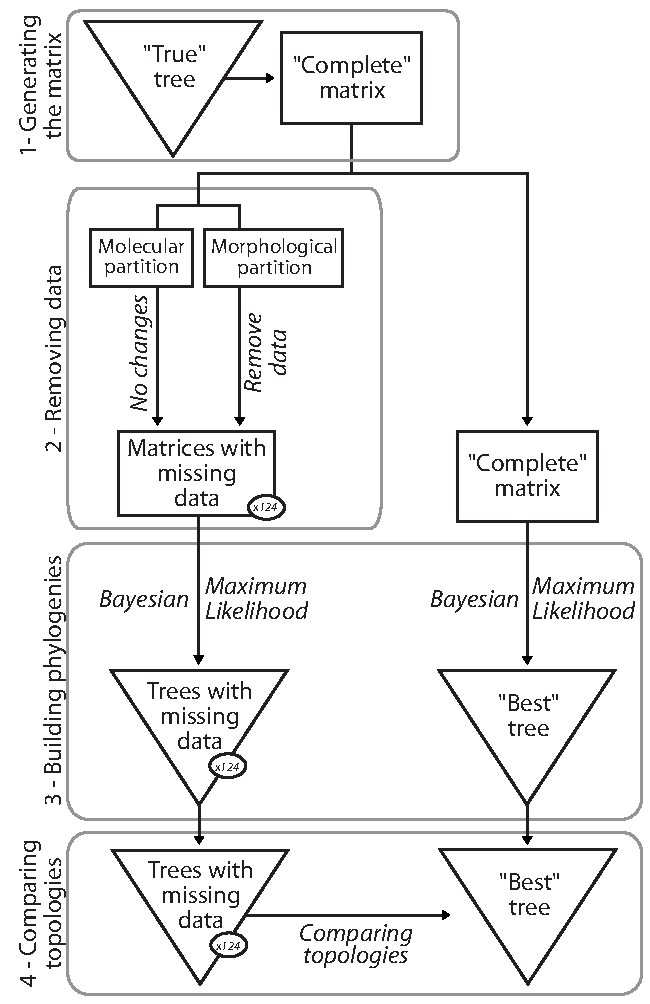
\includegraphics[keepaspectratio=true]{Figures/BW/TEM_Fig_outline-BW.pdf}
\caption{Protocol outline.
(1) We randomly generated a birth-death tree (the "true" tree) and used it to infer a matrix with no missing data (the "complete" matrix).
(2) We removed data from the morphological part of the "complete" matrix resulting in 125 "missing-data" matrices.
(3) We built phylogenetic trees from each matrix using both Maximum Likelihood and Bayesian methods.
(4) We compared the "missing-data" trees to the "best" tree.
We repeated steps 1-4 50 times.}
\label{Fig_Outline}
\end{figure}

%---------------------------------------------
%       Generating the matrix
%---------------------------------------------

\subsection{Generating the matrix}
First we randomly generated a "true" tree of 50 taxa in R v3.0.2 \citep{R302} using the package diversitree v0.9-6 \citep{fitzjohndiversitree2012}. We generated the tree using a birth death process by sampling speciation ($\lambda$) and extinction ($\mu$) rates from a uniform distribution but maintaining $\lambda$ $>$ $\mu$ \citep{paradistime-dependent2011}. We implemented a rejection sampling algorithm to select only trees with 25 living and 25 fossil taxa to ensure that we had enough taxa of each type for our missing data simulations to work. We then added an outgroup to the tree, using the mean branch length of the tree to separate the outgroup from the rest of the taxa, and with the branch length leading to the outgroup set as the sum of the mean branch length and the longest root-to-tip length of the tree.

Next, we generated a molecular and a morphological matrix from the "true" tree. The molecular matrix was inferred from the "true" tree using the R package phyclust v0.1-14 \citep{chen2011}. The matrix contained 1000 character sites for 51 taxa and was generated using the seqgen algorithm \citep{ranbaut1997seqgen} and using the HKY model \citep{HKY85} with random base frequencies and transition/transversion rate of 2 \citep{douadycomparison2003}. The substitution rates were distributed following a gamma distribution with an alpha ($\alpha$) shape of 0.5 \citep{yangamong-site1996}. We chose a low value of $\alpha$ to reduce the number of sites with high substitution rates, thus avoiding too much homoplasy and a decrease in phylogenetic signal. We selected the parameters above to generate data with no special assumption about how the characters evolved, and to reduce the computational time required if these parameters were estimated rather than defined in the tree building part of the analysis (even with the parameters defined, total computational time for the whole analysis was over 150 CPU years). All the molecular information for fossil taxa was replaced by missing data ("?").

We inferred the morphological matrix using the R package ape v3.0-11 \citep{paradisape:2004} to generate a matrix of 100 character sites for 51 taxa. We assigned the number of character states (either two or three) for each morphological character by sampling with a probability of 0.85 for two states characters and 0.15 for three state characters. These probabilities were selected using the overall distribution of character states extracted from 100 published empirical morphological matrices (See \hyperref[SupplementaryMaterial]{Supplementary Material Section 1}). We then ran an independent discrete character simulation for each character using the "true" tree with the character's randomly selected number of states (two or three) and assuming an equal rate of change (i.e. evolutionary rate) from one character state to an other \citep{Pagel22011994}. This method allows us to have only two parameters for each character: the number of states and the evolutionary rate. For each character, the evolutionary rate was sampled from a gamma distribution with $\alpha$ = 0.5. We used low evolutionary rate parameters (i.e. $\alpha$) to avoid homoplasy in the morphological part of the matrix and create a clear phylogenetic signal \citep{wagner2000,davalosintegrating2014}.

Finally, we combined the morphological and molecular matrices obtained from the "true" tree. Hereafter we call this the "complete" matrix: the matrix with no missing data except for the molecular data of the fossil taxa.

%---------------------------------------------
%       Removing data
%---------------------------------------------

\subsection{Removing data}
\label{Removing_data}
We modified the "complete" matrix to get matrices with missing data by randomly replacing data with "?" in the morphological part of the matrices according to the following parameters:% (Fig. ~\ref{Fig_RemoveData}): % PUT IN APPENDIX

\begin{enumerate}
\item{The proportion of living taxa with no morphological data ($M_{L}$): 0\%, 10\%, 25\%, 50\% or 75\%.}
This parameter illustrates the number of living taxa that are present in the molecular part of the matrix but not in the morphological part. This reflects the fact that because of the increasing availability of DNA sequences for living taxa, detailed morphological data is scarce.
\item{The proportion of missing data in the fossil taxa ($M_{F}$): 0\%, 10\%, 25\%, 50\% or 75\%.}
This parameter illustrates the quality of the fossil record. 
\item{the proportion of missing morphological characters for both living and fossil taxa ($M_{C}$): 0\%, 10\%, 25\%, 50\% or 75\%. }
This parameter illustrates the number of available morphological characters for both living and fossil taxa.
\end{enumerate}

In practice, each parameter represents a different way of removing data from the matrix: $M_{L}$ removes rows from the living taxa; $M_{F}$ removes cells from the fossil taxa; and $M_{C}$ removes columns across both living and fossil taxa. Note that $M_{L}$ is different to $M_{F}$ not only because of the region of the matrix affected: for $M_{L}$, all the morphological data of a percentage of living taxa is removed, but for $M_{F}$, a percentage of the data is removed at random from across the whole of the morphological matrix for fossil taxa.

We tested all parameters combinations resulting in 125 ($5^3$) matrices. Note that one of these combinations has no missing data so is equivalent to the "complete" matrix, thus we have one effectively complete matrix in our 125 "missing-data" matrices. Because some parameter combinations introduce a lot of missing data (e.g. $M_L$=75\%, $M_F$=75\% and $M_C$=75\%), some matrices contained fossil taxa without any data at all. When this occurred we repeated the random deletion of characters until every taxa had at least 5\% data across the whole morphological part of the matrix.

%---------------------------------------------
%       Building phylogenies
%---------------------------------------------

\subsection{Building phylogenies}
From the resulting matrices we generated two types of trees, the "best" tree inferred from the "complete" matrix and the "missing-data" trees inferred from the 125 matrices with various amounts of missing data. The "true" tree was used to generate the "complete" matrix and reflects the "true" evolutionary history in our simulations. The "best" tree, on the other hand, is the best tree we can build using state-of-the-art phylogenetic methods. In real world situations, the "true" tree is never available to us because we cannot know the true evolutionary history of a clade (except in very rare circumstances, e.g. \citealt{rozen2005}). Therefore, here we focus on comparing the trees inferred from the matrices with missing data to the "best" tree, rather than the "true" tree, as the "best" tree is generally what biologists have to work with.

\subsubsection{Maximum Likelihood}
The "best" tree and the "missing-data" trees were inferred using RAxML v8.0.20 \citep{Stamatakis21012014}. For the molecular data, we used the GTR + $\Gamma_4$ model (\citealt{tavare1986}; default GTRGAMMA in RAxML v8.0.20; \citealt{Stamatakis21012014}) as a generalization of the HKY + $\Gamma_4$ model \citep{HKY85} for the molecular data.
%The GTR model can be seen as a generalization of the HKY model (the two parameters from the HKY model are implicitly included in the six from GTR model - \citealt{stamatakisa2008}). - TG: Is that useful? 
For the morphological data, we used the implemented Markov \textit{k} state model \citep{lewisa2001} %which is a generalization of the JC69 model \citep{jc69} with \textit{k} $\geq$ 2 - TG: same?
 assuming an equal state frequency and a unique overall substitution rate ($\mu$) following a gamma distribution of the rate variation with four distinct categories (M\textit{k} + $\Gamma_4$; -K MK option in RAxML v8.0.20; \citealt{Stamatakis21012014}).

In order to measure the phylogenetic signal of our simulations, we first ran a fast bootstrap analysis with 500 replicates on the "complete" matrix. We removed all the simulations that had a median bootstrap support lower than 50 as a proxy for weak phylogenetic signal \citep{zanderminimal2004}. We repeated this selection until we obtained 50 sets of simulations (i.e. 50 "complete" and 50*125 "missing-data" matrices) with a relative good phylogenetic signal (median bootstrap $>$ 50).

On these selected simulations, we used the fast bootstrap algorithm and performed 1000 bootstraps per tree inference to assess the topological support \citep{pattengale2010many}.
%The bootstrap algorithm used in RAxML is the Lazy Sub-tree Rearrangement (LSR) which consists of pruning one sub-tree from the tree and subsequently reinserting it to all neighbouring branches \citep{stamatakisa2008}. Sub-tree Pruning and Reinserting methods (SPR) have been demonstrated to be better than other methods (e.g. Nearest Neighbouring Interchange - NNI) for recovering good bootstrap values \citep{salamin2003}. %TG: The explanations of the algorithm part for the BS was proposed by Trevor I think it's useless
When using these parameters, it took 6 CPU years to build 50 sets of 125 bootstrapped Maximum Likelihood trees (8 core nodes 2.30GHz clock speed).

\subsubsection{Bayesian}
The "best" tree and the "missing-data" trees were inferred using MrBayes v3.2.1 \citep{Ronquist2012mrbayes}. We partitioned the data to treat the molecular part as a non-codon DNA partition and the morphological part as a multi-state morphological partition. The molecular evolutionary history was inferred using the HKY model with a transition/transversion ratio of two \citep{douadycomparison2003} and a gamma distribution for the rate variation with four distinct categories (HKY + $\Gamma_4$). For the morphological data, we used the Markov \textit{k} state model \citep{lewisa2001}, with equal state frequency and a unique overall substitution rate ($\mu$) with four distinct rates categories (M\textit{k} + $\Gamma_4$). We chose these models to be consistent with the parameters used to generate the "complete" matrix.

Each Bayesian tree was estimated using two runs of four chains each for a maximum of 50$\times$$1^6$ generations. We used the average standard deviation of split frequencies (ASDS) as a proxy to estimate the convergence of the chains and used a stop rule when the ASDS went below 0.01 \citep{Ronquist2012mrbayes}. The effective sample size (ESS) was also checked on a random sub-sample of runs in each simulation to ensure that ESS $>>$ 200 \citep{drummond2006ess}. For each run, we removed 25\% of the iterations as burn-in. We used the following priors for each tree (see \hyperref[SupplementaryMaterial]{Supplementary Material S1}):
\begin{enumerate}
\item the "true" tree’s topology as a starting tree (with a starting value for each branch length of 1),
\item an exponential prior on the shape of the gamma distribution of $\alpha$ = 0.5 for both partitions, and
\item a transition/transversion ratio prior of two sampled from a strong beta distribution ($\beta$(80,40)).
\end{enumerate}

We used these prior to speed up the Bayesian estimation process. These priors biased the way the Bayesian process calculated branch lengths by giving non-random starting points and boundaries for parameter estimation, however, here we are focusing on the effect of missing data on tree topology and not branch lengths. Even using these priors, it took 140 CPU years to build 50 sets of 125 Bayesian trees (8 core nodes 2.30GHz clock speed).

%---------------------------------------------
%       Comparing Topologies
%---------------------------------------------

\subsection{Comparing topologies}
We compared the topology of the "missing-data" trees to the "best" tree to measure the effect of the three parameters $M_{L}$, $M_{F}$ and $M_{C}$ on tree topology. We used the Robinson-Foulds distance \citep{RF1981} to identify conserved clade positions and the Triplets distance \citep{dobson1975triplets} to assess the number of conserved taxa across trees. We then used Normalized Tree Similarity index \citep{Bogdanowicz2012} to generalize our results for any \textit{n} number of taxa. These metrics are described in detail below.
%ADD KHUNAR PAPER SOMEWHERE

\subsubsection{Robinson-Foulds distance}
Robinson-Foulds distance \citep{RF1981}, or "path difference", measures the number of shared clades across two trees. The metric reflects the distance between the distributions of tips among clades in the two trees (\citealt{RF1981} ; see \hyperref[SupplementaryMaterial]{Supplementary Material S2}). This metric is bounded between 1 when the two trees are identical and $n-2$ (for two trees with $n$ taxa) when there is not one single shared clade between both trees. This metric is sensitive to the exact clade conservation: if the trees are composed of two clades of three taxa (\textit{(((a,b),c),((d,e),f))}), the swap of two taxa will lead to a maximal score of the Robinson-Foulds distance indicating a bad tree similarity.

\subsubsection{Triplets distance}
The Triplets distance \citep{dobson1975triplets} measures the number of sub-trees made up of three taxa that differ between two given trees (\citealt{critchlowthe1996} ; see \hyperref[SupplementaryMaterial]{Supplementary Material S2}). This metric measures the position of each taxon and clade towards it's closest neighbours. It is bounded between 0 when the two trees are identical and $\binom{n}{4}$ (for two trees with $n$ taxa) when there is not one single position of taxon/clade identical between both trees. Therefore this metric sensitive to the conservation of individual taxa towards the neighbouring trees.

\subsubsection{Normalized Tree Similarity}
We used the Normalized Tree Similarity index, $NTS_m$ (\citealp{Bogdanowicz2012}) to be able to compare the two metrics for any $n$ taxa. This index allows to scale the value of any metric $m$ (either Robinson-Foulds or Triplets distance in our study) to the expected value of the metric $m$ when comparing two random trees (see \hyperref[SupplementaryMaterial]{Supplementary Material S2}). When $NTS_m$=1, the two trees are strictly identical, when $NTS_m$=0 the trees are no more different than expected when comparing two random trees and when $NTS_m$$<$0, the difference between the two trees is greater than when comparing two random trees. In our study we used the $NTS_m$ index as a proxy for topology: a high score of this index (i.e. towards 1) means that the topology is highly conserved between the two trees; on the opposite, a low score of this index (i.e. towards 0) means that the topological difference between the two trees is as much as expected when comparing two random trees. Note that both tree comparisons are representing different aspects of topological similarity and do not perform equaly (see \hyperref[metrics_discussion]{discussion below} and \citealt{kuhnerpractical2014}).

\subsubsection{Tree comparisons}
\label{tree_comparisons}
For the Maximum Likelihood and Bayesian consensus trees we performed pairwise comparisons between the "best" tree and each "missing-data" tree using both the Robinson-Foulds and Triplets metrics with the TreeCmp java script \citep{Bogdanowicz2012}. For each metric, we then normalized the value using the Normalized Tree Similarity scaled by the mean value of 1000 pairwise random tree comparisons for the metric in question and n = 51 taxa (see \hyperref[SupplementaryMaterial]{Supplementary Material Section 2}). % TG: Maybe remove supplementary here
We compared each "missing-data" tree with the "best" tree for each of our 50 simulation runs resulting in 50 comparisons for each "missing-data" tree. We calculated the mode and the 50\% and 95\% confidence intervals from the resulting distribution using the hdrcde R package v3.1 \citep{hdrcde}.

Also, to take into account the uncertainty of tree inference in both Maximum Likelihood and Bayesian (i.e node support), we ran 1000 random pairwise comparison between respectively the bootstrapped trees from the Maximum Likelihood analysis and the posterior tree distribution of the Bayesian analysis. In the same way that we compared a single "missing-data" tree to the "best" tree (whether the trees are Maximum Likelihood or Bayesian consensus): we randomly selected 1000 trees from the "missing-data" tree sets (either the Bootstrapped trees or the posterior tree distribution) and did a pairwise comparison with 1000 randomly selected trees from the "best" tree set.

For each of the 125 "missing-data" tree, we obtained Robinson-Foulds and Triplets distance distributions from either 50 or 50*1000 pairwise comparisons. We then calculated the mode and the 50\% and 95\% confidence intervals from the resulting distribution using the hdrcde R package v3.1 \citep{hdrcde}. %Finally we tested for significant differences among the different distributions of trees using non-parametric group and pairwise comparisons by using respectively Kruskal-Wallis and Nemenyi-Damico-Wolfe-Dunn test (CITE R PACKAGE)\citet{ruxtontime2008}.

In order to investigate the effect of the parameters and/or the methods used in this simulations, we measured the similarity among the different distributions using the Bhattacharyya Coefficient \citep{Bhattacharyya}. The Bhattacharyya Coefficient is the probability of overlap between two distributions, ranging from 0 to 1 (\citealt{Bhattacharyya} - see \hyperref[SupplementaryMaterial]{Supplementary Material Section 2}). For each method (Maximym likelihood trees, Bayesian consensus trees, Bootstraps and Bayesian posterior trees) and metric (Robinson-Foulds and Triplets distance), we used this coefficient in two ways in order to:
\begin{enumerate}
\item assess the effect of the method on all parameters:

We performed a pairwise comparison of each parameter between each pair of methods. This resulted in 125 comparisons per method and per metric (each parameter combination within one method compared to the same parameter combination in the other method). We then compared the distribution of these pairwise comparisons to see the global difference between two methods: if the method have really similar results, we would expect the distribution to be cluster around 1 (high probability of overlap between the distributions) and if the methods are really dissimilar around 0 (low probability of overlap - Fig.~\ref{Fig_Results-paircomp_without}).
\item assess the effect of the parameters within a method:

We performed a pairwise comparison per method and per metric for each combination of parameters. This resulted in 7875 pairwise comparisons per method and per metric (triangle of a 125*125 matrix). We represented these results as a triangular matrix with the values of each pairwise comparison coloured according to the value of the Batthacharyya Coefficient (coloured in green when the distributions overlap completely and in red when they don't - Fig.~\ref{Fig_Results-paircomp_within}).
\end{enumerate}

%---------------------------------------------
%
%       RESULTS
%
%---------------------------------------------

\section{Results}

\subsection{Effect of missing data on topology}

\begin{figure} 
\centering
    \includegraphics[width=1\textwidth]{Figures/colour/Parameters-AllMethods-RF+Tr-small.pdf}
\caption{Comparison between the effect of missing data and the tree inference method on topology. The amount of missing data for each parameter is represented on the x axis. The topology is represented on the y axis, both using Robinson-Foulds distance (upper row) and Triplets distance (lower row). Points represent the modal value of each distribution ; thick solid and thin dashed lines represents respectively the 50\% and 95\% confidence intervals or the distributions. The Maximum Likelihood trees are represented in black, the Bayesian consensus trees in red, the bootstrap trees in green and the posterior tree distribution in blue.}
\label{Fig_Results-permeth_perparam} %Differences within a subset of parameters and between methods
\end{figure}

As it would be expected form the literature, the amount of missing data in the morphological matrix does decrease the ability to recover the right topology, regardless of the parameter, the method or the metric used \citep[e.g.][]{rouresite-specific2011,sansomfossilization2013,pattinsonphylogeny2014}. However each variable does not affect the topology in the same way (Fig.~\ref{Fig_Results-permeth_perparam}). Regarding the conservation of entire clades (i.e. the Ronbinson-Foulds distance), the Bayesian consensus trees outperform the other methods and the amount of missing data in the living taxa ($M_{L}$) decreases the most rapidly the clade conservation when using this method. However, when looking at the position of wild card taxa (i.e. the Triplets distance), the Maximum Likelihood outperforms the other methods but with wider distributions overlap (Fig.~\ref{Fig_Results-paircomp_without}-B).

\begin{figure} 
\centering
    \includegraphics[width=1\textwidth]{Figures/BW/Global-ML+consensus-RF+Tr-small.pdf}
\caption{Trend of the effect of missing data on topology on ML and consensus trees. The amount of missing data per parameter ($M_{L}$, $M_{F}$ and $M_{C}$) is represented along the x axis. The colour gradient from white to black represents respectively, 0\%, 10\%, 25\%, 50\% and 75\% of missing data. The topology is represented on the y axis, both using Robinson-Foulds distance (upper row) and Triplets distance (lower row). Points represent the modal value of each distribution ; thick solid and thin dashed lines represents respectively the 50\% and 95\% confidence intervals or the distributions. The Maximum Likelihood trees are represented in black and the Bayesian consensus trees in grey.}
\label{Fig_Results-global_perparam} %Differences between all the parameters and between two methods (ML vs BC)
\end{figure}

When looking at the global trend of the Bayesian consensus trees for all the parameters combinations, this method outperforms Maximum Likelihood for the Ronbinson-Foulds distance and plateaus to a minimal modal tree similarity of 0.69 regardless the amount of missing data (Fig.~\ref{Fig_Results-global_perparam} - see also \hyperref[SupplementaryMaterial]{Supplementary Material Section 3}). However, regarding the Triplets distance, Bayesian consensus trees seems to perform poorly but with great confidence intervals overlaps (Fig.~\ref{Fig_Results-global_perparam} and Fig.~\ref{Fig_Results-paircomp_within}). These greater larger confidence intervals are due to the lower ability of the Triplet method to highlight precise differences in topology \citep{kuhnerpractical2014}. Results for the global trend comparison between the uncertainty methods (Bootstrap and Bayesian posterior tree distribution) are available in the supplementary materials (see \hyperref[SupplementaryMaterial]{Supplementary Material Section 3}).

\subsection{Effect of the method on topology}

\begin{figure} 
\centering
    \includegraphics[width=1\textwidth]{Figures/colour/PairComp_without-RF+Tr.pdf}
\caption{Distribution of the Bhattacharyya Coefficients between methods. Curves represents the kernel density estimations of the BC between the four different methods. A. Results for the Normalised Robinson-Foulds distance. B. Results with the for Normalised Triplets distance. Pikes around the two different extremes values of the BC show the two pairs of most dissimilar methods (Bayesian consensus vs. Bootstraps and Bayesian consensus vs. Bayesian posterior trees) for the Normalised Robinson-Foulds distance ; and the most similar methods (Bootstraps and Bayesian posterior trees) for the Normalised Triples methods.}
\label{Fig_Results-paircomp_without} %Comparisons between methods, both in RF and Triplets.(method differences)
\end{figure}

When looking at the comparisons between the methods using the Robinson-Foulds distance, the Bayesian consensus trees have the least overlap with respectively the Bayesian posterior trees and the Bootstrap (Fig.~\ref{Fig_Results-paircomp_without}-A). When regarding at the Triplets distance, the two method that have the most distribution are the Bootstraps and the Bayesian posterior trees (Fig.~\ref{Fig_Results-paircomp_without}-B). These results are due to the slight difference in comparing topologies between Maximum Likelihood and Bayesian consensus trees and Bootstraps and Bayesian posterior trees: the two last ones are based on a random pairwise comparison of a sub-sample of 1000 trees. This is likely to add noise to the data.

\subsection{Effect of the missing data parameters on topology}

\begin{figure} 
\centering
    \includegraphics[width=1\textwidth]{Figures/colour/PairComp_within-Baycon-RF+Tr.pdf}
\caption{Pairwise Bhattacharyya Coefficients within the Bayesian consensus trees. The pairwise trees comparisons are represent on both axis. The colour gradient from white to black represents respectively, 0\%, 10\%, 25\%, 50\% and 75\% of missing data. The matrix represents the values of pairwise Bhattacharyya Coefficients going from green (BC=1) to red (BC=0). A. Results for the Normalised Robinson-Foulds distance. B. Results with the for Normalised Triplets distance.}
\label{Fig_Results-paircomp_within}
\end{figure} %Pairwise BC for the Bayesian consensus trees for RF and TR. (parameters differences)

When looking at the pairwise Bhattacharyya Coefficients between all the parameters combinations for Bayesian consensus trees, the number of missing living taxa ($M_{L}$) results the lowest probabilities of overlap (right lower corner in Fig.~\ref{Fig_Results-paircomp_within}-A). However, when looking at the Triplets distance, because of the high overlap in confidence intervals, there is no major region with low probability of overlap. One should note however that the bottom line of the matrix where the Bhattacharyya Coefficients are very low is due to comparing the distribution of the pairwise comparison of the best tree vs. the best tree, leading to a Normalised triplet score of 1 every time (with no variance, see Fig.~\ref{Fig_Results-permeth_perparam} and Fig.~\ref{Fig_Results-global_perparam}). All the other pairwise comparisons are available in the supplementary materials (see \hyperref[SupplementaryMaterial]{Supplementary Material Section 3}).

%---------------------------------------------
%
%       DISCUSSION
%
%---------------------------------------------

\section{Discussion}

% NC: Discussions usually begin with a paragraph that sums up the results. Then you can move on to discussing caveats, problems, extensions etc. You also need to show how your work fits in with the wider literature. So I think you need to re-write this completely with that in mind. Do the same as we did for the introduction - write a line for each paragraph. This reads like you jumped in without thinking clearly about the structure. It probably doesn't need to have all the same subheadings either.

%§1
%Results: global
%   -Missing data increase decreases topological recovery
The results of our simulations are in adequacy with recent analysis on the effect of missing data in morphological matrices \citep{pattinsonphylogeny2014,wrightbayesian2014,sansombias2014}. Our results are showing that ability to recover the correct topology decreases with the amount of missing data, regardless the metric, the method or the parameters considered.
%Results 1
%   -However, parameters have different effect
However, within a method and a metric, the parameters used to remove data have different effects on the ability to recover the correct topology.
%Results 2
%   -Additionally, methods and metrics are unequal
Additionally, the effect of missing data on topological recovery varies with different methods to infer topology and different metrics to compare topologies.
%Wrap up results
%   -Thus, Baycon is better with loads of living 
Thus, we found that using the topologies of Bayesian consensus trees performed consistently better than other methods for recovering the correct topology (Fig.~\ref{Fig_Results-global_perparam} and Fig.~\ref{Fig_Results-paircomp_within}) and that both the amount of available characters ($M_{C}$) and the amount of data for the living taxa ($M_{L}$) are crucial missing data parameters (Fig.~\ref{Fig_Results-paircomp_within}).

%§2
%Results 1 from litterature
%   -Missing data per se is not a problem, problem is in the amount of overlap
As proposed in previousstudies, the amount of missing data is not a problem \textit{per se} as long as enough data overlaps in the matrix \citep[e.g.][]{kearneyfragmentary2002,wiensmissing2003,rouresite-specific2011,pattinsonphylogeny2014}. %In fact, as shown previously, the amount of overlap in the matrix is more crucial than the proportion of missing data \citep[e.g.][]{rouresite-specific2011}.
%Proposed hypothesis for result 1
%   -One can increase overlap by adding living taxa
To improve topological recovery in a Total Evidence framework, one can efficiently increase the amount of overlapping data by reducing the amount of missing data in each of our three selected parameters. In our simulations, the overlap in data is greatly reduced when different parameters are combined with a high amount of missing data (e.g. $M_{L}$=75\%, $M_{F}$=75\% and $M_{C}$=75\% - Fig.~\ref{Fig_Results-permeth_perparam} and Fig.~\ref{Fig_Results-global_perparam}). In this scenario the overall number of missing characters ($M_{C}$) affects the proportion of overlapping data by reducing the overall size of the matrix (Fig.~\ref{Fig_Results-global_perparam}). However it is important to note that in the pairwise Bhattacharyya Coefficient analysis, the area with the lowest probability of distributions overlap is led by comparing the trees with no missing data for the living taxa to the trees with 75\% missing data for the living data (right lower corner in Fig.~\ref{Fig_Results-paircomp_within}).

%§3
%Discussing results 1
Each of our parameters illustrate one potential source of missing data in a morphological matrix (see \hyperref[Removing_data]{Methods}). We have suggestions for practical ways to reduce the missing data problem:
%   -Which parameters does what?
\begin{enumerate}
\item{$M_{L}$ (non coded living taxa):}
The vast majority of known living species have specimens preserved in natural history museums. This is a significant resource and more research effort is needed to code morphological characters in these specimens.
\item{$M_{F}$ (quality of the fossil record):}
The amount of missing data in the fossil record solely depends on the preservation quality of the fossils and can not be actively improved. However, gaps in the matrix can be filled with the discoveries exceptional preserved fossil \citep[e.g.][]{nithe2013}. Fortunately, this parameter is the most difficult to improve but it also has the least influence on whether the simulations recover the correct topology (Fig.~\ref{Fig_Results-paircomp_within}).
\item{$M_{C}$ (amount of coded characters):}
The amount of time it takes to build a morphological matrix increases directly with the number of characters involved. Improvement in both decreasing the time taken to build the matrix and increasing the number of characters can be done through vast collaborative data collection projects through web portals such as \textit{morphobank} \citep{morphobank}.
\end{enumerate}


%§4
%Result 2 from literature.
%   -Probabilistic method always better (wright but see spencer) - Check McGuire[nope]/Sean[nope] literature for Bayesian vs. ML?
Nonetheless, as our results shows in Fig.~\ref{Fig_Results-permeth_perparam} and Fig.~\ref{Fig_Results-global_perparam}, the variation in the ability to recover the correct topology does not only depend on the missing data in morphological part of the matrix but also heavily on the method used to infer the topology. Previous studies have shown some superiority on methods using simple probabilistic models such as the M\textit{k} model \citep{lewisa2001} over cladistic methods (\citealt{wrightbayesian2014} but see \citealt{spencerefficacy2013}). However, this is the first study, to our knowledge, that compares the performance of the M\textit{k} model \citep{lewisa2001} between Maximum Likelihood and Bayesian inference in a Total Evidence framework. %TG: I do have to check the Mk in Baysian vs Mk in ML part though but I guess it's a good selling point: we ARE the first ones to do a sensitivity analysis in a TEM framework (as far as we know).
%Discussing results 2
%   -Why is Baycon better than the others?
When using the clade conservative Robinson-Foulds distance (see \citealt{kuhnerpractical2014} and \hyperref[metrics_discussion]{discussion below}), the Bayesian consensus trees greatly outperforms the Maximum Likelihood trees in the ability to recover the correct tree topology (Fig.~\ref{Fig_Results-global_perparam}). In fact, regardless of the amount of missing data, this method always displays the highest normalised Robinson-Foulds score (always $>$ 0.69 - see \hyperref[SupplementaryMaterial]{Supplementary Material Section 3}). Also, when looking at the pairwise Bhattacharyya Coefficients within each method, the Bayesian consensus tree one display the highest probability of overlap between the results in any case (see \hyperref[SupplementaryMaterial]{Supplementary Material Section 3}).

%   -Why is Baycon so different than Baytre? Since Baycon is calculated from Baytre.
When comparing this the probability of overlap between the methods, it is counter intuitive to note that the Bayesian consensus tree shows the highest dissimilarity with the Bayesian posterior trees from which the consensus tree is build (Fig.~\ref{Fig_Results-paircomp_within}-A). Note that it is also highly dissimilar to the Bootstraps. However that can be linked to the fact that both Bootstraps and Bayesian posterior trees are measured as 125*1000 random pairwise comparisons instead of just 125 tree comparisons for the Bayesian consensus trees. The fact that the 1000 pairwise trees to be compared for each of the 125 comparisons are chosen randomly, it can add noise to the results for these two methods (see \hyperref[tree_comparisons]{methods above}).

%Some sort of transition?

%§5

%Caveats: the metrics
%   -RF is different and better than triplets.
\label{metrics_discussion}
As shown in Fig.~\ref{Fig_Results-permeth_perparam} and Fig.~\ref{Fig_Results-global_perparam}, our results can be contrasted by looking at the normalised tree similarity when using the Robinson-Foulds or the Triplets distance. For example, Fig.~\ref{Fig_Results-global_perparam} shows opposite results for both method when looking at the two different metrics. Globally, the normalised Triplets distance displays large confidence intervals than the normalised Robinson-Foulds distance and a higher probability of overlap between the distribution of each parameter (Bhattacharyya Coefficient close to 1 - Fig.~\ref{Fig_Results-paircomp_within}-B). The contrast between the results of the two metrics can be explained by the actual nature of both metrics (see \hyperref[SupplementaryMaterial]{Supplementary Material S2}):
\begin{enumerate}
\item{The Robinson-Foulds metric is a conservative metric, it is more sensible to single taxon displacement because it will count clades as similar only if they are composed of the same taxa with the same topologies \citep{RF1981}. When getting closer to the root of the tree, displacement of single taxon makes the clades not being exactly identical any more even if the clade still contains all the other taxa in both trees. This metric illustrates therefore the conservation of clades among the compared trees (i.e. when the normalised Robinson-Foulds distance is close to 1, most of the clades in the two trees are identical).}
\item{On the other hand, the Triplets method is measuring the position of each taxon towards two other reference taxa \citep{critchlowthe1996}. It will penalise only trees where taxa get removed furthest from their original position. This metric therefore illustrates the amount of wildcard taxa \citep{kearneyfragmentary2002} between the to compared trees (i.e. when the score is closed to 1, few wildcard taxa are present in the tree).}
\end{enumerate}
Therefore, in our study, both metrics are showing two different aspects of tree topology. For example, regarding the Bayesian consensus trees, completes clade are conserved most of the time (Fig.~\ref{Fig_Results-global_perparam}-top) but with increasing amount of missing data, wildcard taxa get more and more displaced (Fig.~\ref{Fig_Results-global_perparam}-bottom). Because we are comparing the Baysian consensus tree to a single tree topology, the probability of recovering the exact position of a wildcard taxa than in the "best" tree is really low and even reducing with the amount of missing data. Regarding this fundamental differences, the Robinson-Foulds metric performs better in showing a distance from the true topology than the Triplets distance \citep{kuhnerpractical2014}.

%§6
%Caveats: the simulations
%   -Simulating morpho characters
Another caveat of our analysis is the performance of our simulation protocol: in order to reduce the computational time ($~$150 CPU years) of our analysis, we had to simulate modest size matrices (1000 molecular data and 100 morphological data) that are two orders of magnitude lower than some matrices used in published analysis: both for the molecular part \citep[e.g.][]{springermacroevolutionary2012} and the morphological part \citep[e.g.][]{nithe2013}. %TG: note about NOT citing O'Leary here. 1-I don't like the paper ; 2-the Ni et al paper (primates) as a big morpho matrix too (1k  characters against 4k for O'Leary, same order of magnitude?) ; 3-We might want to limit the papers we're citing?
Also, simulating morphological characters is more complex than molecular ones. The underlying pattern of their evolution are often more complex and ruled by more parameters than molecular characters (i.e the number of character states, the states frequencies, the substitution matrix and the statistical model used) \citep{Pagel22011994,wagner2000,lewisa2001}. Also morphological characters studies involve many potential statistical pitfalls (e.g. independent characters violation, rate variation - \citet{davalosintegrating2014}) and especially (i) incongruence with molecular signal and (ii) homoplasy \citep{wagner2000}.
\begin{enumerate}
\item{First, morphological data can display a different signal than molecular data, especially in small matrices. %REF
This might lead to a controversial phylogenetic signal in the overall matrix and lower down the support values. However, regarding empirical data studies, most of the groups shows fairly congruent morphological and molecular phylogenetic signal \citep[e.g.][]{leerates2013}.}
\item{Secondly, in this study, we made the assumption that theoretically, morphological characters are randomly distributed on an organism however it seems clear that empirical morphological data does not act randomly \citep{sansomfossilization2013,pattinsonphylogeny2014}. However, following our simulation assumption of random character distributions, if they accumulate through time in the same way as the majority of the molecular characters then, homoplasic characters are expected to appear randomly through time \citep{davalosintegrating2014}. Therefore, homoplasy is expected to be more important (by chance) in bigger morphological matrices \citep{davalosintegrating2014}. After reaching a critical amount of morphological characters, adding new ones increases homoplasy \citep{wagner2000}.}
\end{enumerate}

%§7
%Further directions - is that necessary though?
%   -Using real data
One way to address this issue would be to run a similar analysis using real data. The amount of studies using Total Evidence data type matrices is steadily increasing \citep[e.g.][]{ronquista2012,slaterphylogenetic2013,beckancient2014} and one could analysis these total evidence matrices in the same framework as this study. However, the true topology (obtained from a matrix with no missing data) is unlikely to be known. A second way to address this issue, and especially to incorporate the variation of signal in morphological character would be to simulate morphological at different rates \citep{wrightbayesian2014} or to apply patterns of missing data directly obtained from the fossil record \citep{pattinsonphylogeny2014}. Nevertheless, our simulation, by simplifying an ideal world, already show clear results of the effect of missing data on topology in a Total Evidence framework. Also, our results show how recovering the correct topology can be improved by using Bayesian consensus trees in combination with a maximum amount of characters and a of living taxa with morphological data.
%   -Looking at branch length?

%§8
%Back to the importance of TEM
%   -Data is not a major problem
%   -Good and promising method.


%---------------------------------------------
%
%       CONCLUSION
%
%---------------------------------------------

\section{Conclusion} %Can probably just be the last paragraph but I like it to be separated as the take home message

%§Conclusions
%   -TEM works with missing data
%   -Use bayesian consensus
%   -Go code living taxa
Using Total Evidence matrices with missing data is not a problem for recovering the correct topology as long as enough morphological data is overlapping between the fossil and living taxa. In order to optimize good topological recovery, we propose to use the Bayesian consensus tree over the Maximum Likelihood tree or over a random subset of the Bayesian posterior trees distribution. Also, in order to improve the overlap in data in the morphological part of the matrix, we advice to use all the morphological characters available and to code them for a maximum of living taxa present in the matrix.


%---------------------------------------------
%
%       ...
%
%---------------------------------------------
\section{Supplementary material}
Supplementary material (code, analysis and full results) can be found in the Dryad data repository at http://dx.doi.org/10.5061/dryad.XXXX. %section and sentence format asked by Syst. Biol.

\section{Acknowledgements}
Thanks to Fr\'{e}d\'{e}ric Delsuc, Emmanuel Douzery, Andrew Jackson, Gavin Thomas, April Wright and the members of the Macro Journal Club %TG : Not sure how many people we have to thank but it could also include Graham Slater, Nick Matzke and Trevor Hodkinson.
for useful comments on our simulation protocol.
%Thanks to Sive Finlay, Kevin Healy and Adam Kane for comments on the manuscript. %TG: or helping writing sentences does not really count.
Thanks to Paddy Doyle, Graziano D'Innocenzo and Sean McGrath for assistance with the computer cluster. Simulations used the Lonsdale cluster maintained by the Trinity Centre for High Performance Computing and funded through grants from Science Foundation Ireland. This work was funded by a European Commission CORDIS Seventh Framework Programme (FP7) Marie Curie CIG grant (proposal number: 321696).

%cite cheat sheet
 % The \cite command functions as follows:
 %   \citet{key} ==>>                Jones et al. (1990)
 %   \citet*{key} ==>>               Jones, Baker, and Smith (1990)
 %   \citep{key} ==>>                (Jones et al., 1990)
 %   \citep*{key} ==>>               (Jones, Baker, and Smith, 1990)
 %   \citep[chap. 2]{key} ==>>       (Jones et al., 1990, chap. 2)
 %   \citep[e.g.][]{key} ==>>        (e.g. Jones et al., 1990)
 %   \citep[e.g.][p. 32]{key} ==>>   (e.g. Jones et al., p. 32)
 %   \citeauthor{key} ==>>           Jones et al.
 %   \citeauthor*{key} ==>>          Jones, Baker, and Smith
 %   \citeyear{key} ==>>             1990

\bibliographystyle{sysbio}
\bibliography{References}

%---------------------------------------------
%
%       Supplementary, separated
%
%---------------------------------------------

%Ignore for fast pdf building
\section{Supplementary Material}

    \documentclass[12pt,letterpaper]{article}

%Packages
\usepackage{pdflscape}
\usepackage{fixltx2e}
\usepackage{textcomp}
\usepackage{fullpage}
\usepackage{natbib}
\usepackage{float}
\usepackage{latexsym}
\usepackage{url}
\usepackage{epsfig}
\usepackage{graphicx}
\usepackage{amssymb}
\usepackage{amsmath}
\usepackage{bm}
\usepackage{array}
\usepackage[version=3]{mhchem}
\usepackage{ifthen}
\usepackage{caption}
\usepackage{hyperref}
\usepackage{amsthm}
\usepackage{amstext}
\usepackage{enumerate}
\usepackage[osf]{mathpazo}
\usepackage{dcolumn}
\usepackage{lineno}
\pagenumbering{arabic}


%Pagination style and stuff
\linespread{2}
\raggedright
\setlength{\parindent}{0.5in}
\setcounter{secnumdepth}{0} 
\renewcommand{\section}[1]{%
\bigskip
\begin{center}
\begin{Large}
\normalfont\scshape #1
\medskip
\end{Large}
\end{center}}
\renewcommand{\subsection}[1]{%
\bigskip
\begin{center}
\begin{large}
\normalfont\itshape #1
\end{large}
\end{center}}
\renewcommand{\subsubsection}[1]{%
\vspace{2ex}
\noindent
\textit{#1.}---}
\renewcommand{\tableofcontents}{}
\bibpunct{(}{)}{;}{a}{}{,}

\section{Code}
All code for performing the analyses is available at: \url{https://github.com/TGuillerme/Total_Evidence_Method-Missing_data}.

\newpage
\section{Appendix 1: Tree Building}
  \section{Supplementary material Section 1}

\subsection{Morphological characters states}
In order to obtain a realistic probabilistic value for of \textit{k} characters states for each simulated morphological character, we downloaded 100 random morphological characters (with more than 100 characters each) from TreeBASE database (http://treebase.org/) published between 1985 and 2013 and covering 19 taxomomic classess (Chordata, Arthropoda, Annelida, Angiosperm, Gymnosperm and Pteridophyta).
We selected a total of 22563 characters ranging from 2 to 10 states.
We calculated the proportion of characters with 2, 3, 4, 5, 6, 7, 8, 9 or 10 states.
We then sampeled 22563 \textit{k} values between 2 and 10 with the same proportion of characters from the empirical data.
We then used a simple t-test to check if our simulation was equal to the empirical data.
In this study, we only simulated characters with 2 or 3 states because of the high proportion of ordered characters ecountered on characters with more than 3 states and the difficulties of simulate biologicaly sensible ordered characters.

\begin{figure}
\centering
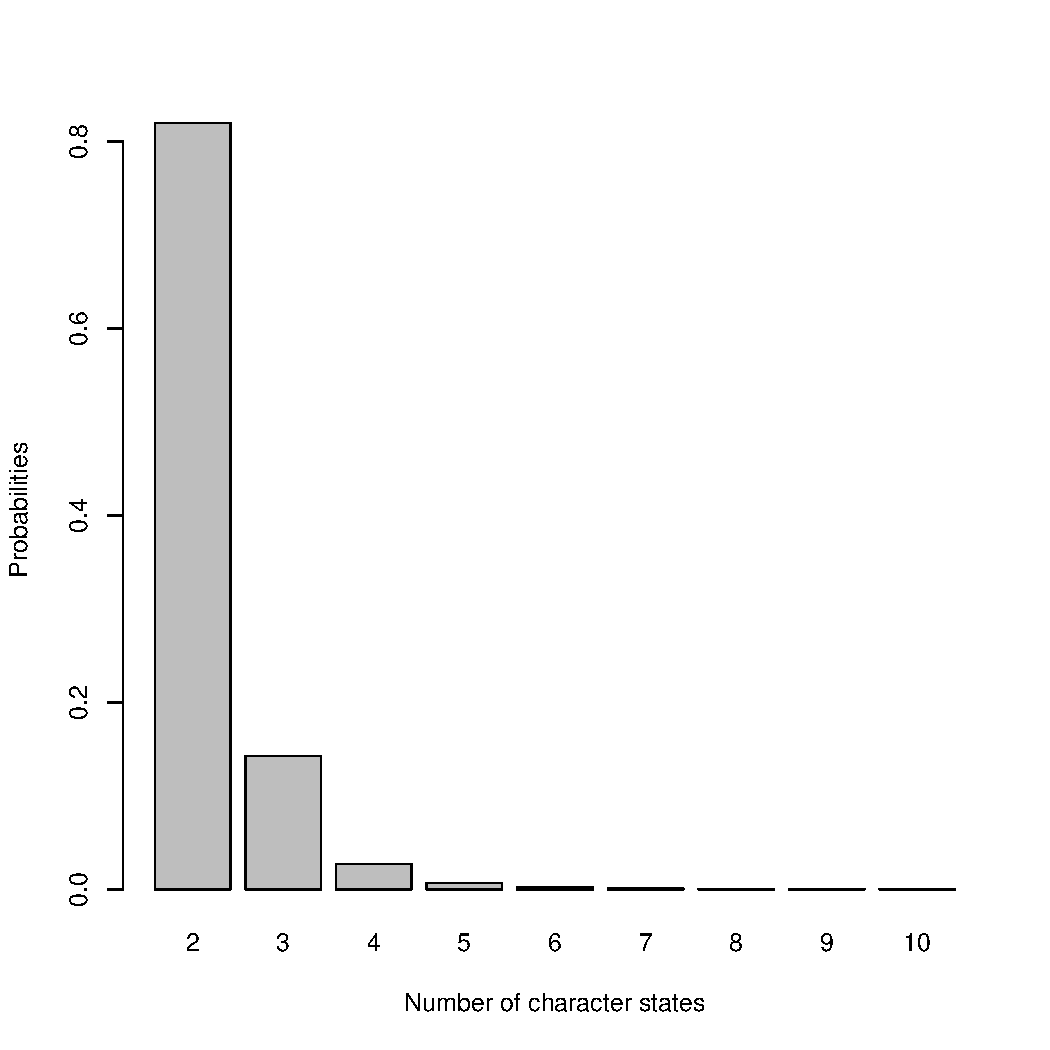
\includegraphics[keepaspectratio=true]{Figures/Supplementary/TEM_Fig-AppendixCharacters.pdf}
\caption{Character states distribution in empirical matrices. %Title?
Characters states number distribution extracted from 100 random morphological matrices downloaded from RreeBase.}
\label{Fig_AppendixCharacters}
\end{figure}


\subsection{Tree Building Software settings}

\subsubsection{Maximum Likelihood - RAxML v8.0.20 \citep{Stamatakis21012014}}

Model: \\
Molecular data: \\
GTR + $\Gamma_4$ (-m GTRGAMMA) \\
Morphological data: \\
Mk + $\Gamma_4$ (-K MK) \\
Support: \\
Rapid Boostrap algorithm (LSR), 1000 replicates \\

\subsubsection{Bayesian - MrBayes v3.2.1 \citep{Ronquist2012mrbayes}}

Priors: \\
Molecular data: \\
rates distribution shape ($\alpha$) = 0.5 \\
Transition/Transversion ratio = 2 ($\beta$(80,40)) \\
Starting tree: "True" tree topology with each branch length = 1 \\
Morphological data: \\
rates distribution shape ($\alpha$) = 0.5 \\
Models: \\
Molecular data: HKY + $\Gamma_4$ \\
Morphological data: Mk + $\Gamma_4$ \\
MCMC: \\
2 runs \\
4 chains per run \\
generations < 50$\times$$1^6$ \\
sample frequency = 1050$\times$$1^3$ \\
ASDS diagnosis frequency = 50$\times$$1^3$ \\
ASDS $<$ 0.01 \\
ESS $>>$ 200 \\
Burnin = 25\%
  \label{Supp_TreeBuilding}

\newpage
\section{Appendix 2: Tree Comparisons}
  %\section{Supplementary material Section 2}

\subsection{Robinson-Foulds distance}
Robinson-Foulds distance (\textit{RF}; \citealp{RF1981}), or "path difference", measures the number of shared clades across two trees. The metric reflects the distance between the distributions of tips among clades in the two trees \citep{RF1981} and can be expressed as:
\begin{equation}
RF_{x,y} = N_{x} + N_{y} - 2C_{x,y}
\end{equation}
where $C_{x,y}$ is the number of clades in common in the two trees. $C$ is equal to one if the two trees have the same $n$ taxa; and $C = n-2$ when none of the $n$ taxa are shared between the trees. This metric is more sensitive to taxon displacement than Triplets distance (i.e. if one taxon moves out of a clade, then the clades are no longer considered similar; \citet{critchlowthe1996,johnson1998,wiensmissing2003}). The minimal value of $C$ is equal to 1 if the two trees have the same n taxa; the maximal value in $C = n-2$. For a fully unresolved tree (star tree) $N$=1 and for a fully resolved tree (binary tree) $N = n-2$. The minimal and maximal topological distance for taxa is:
\begin{equation}
RF_{min} = 1 + 1 - 2C_{x,y}
\end{equation}
and:
\begin{equation}
RF_{max} = 2(n-2)-2
\end{equation}
One can then rescale \textit{RF.scaled} by using the maximal and minimal value for any $n$ taxa:
\begin{equation}
RF.scaled_{x,y} = \frac{RF_{x,y}-RF_{max}}{RF_{max}}
\end{equation}
This metric is more sensitive to taxa displacement than the Triplets distance \citep{critchlowthe1996,johnson1998,wiensmissing2003} and therefore a low value will show a good clade conservation between two trees and a high value will show a bad recovery of common clades.

\subsection{Triplets distance details ($T_{x,y}$)}
Triplets distance ($T_{x,y}$; \citealp{dobson1975triplets}) measures the number of sub-trees made up of three taxa (triplets) that differ between two given trees. Each triplet can be written as $I_{ijk}$=(\textit{ijk}). Where $I_{ijk}$ is equal to zero if the the two triplets (\textit{ijk}) are the same in the two trees otherwise $I_{ijk}$ is equal to one. For any rooted binary tree there are only three possible combinations for each triplet: ((\textit{j},\textit{k}),\textit{i});, ((\textit{i},\textit{k}),\textit{j}); and ((\textit{i},\textit{j}),\textit{k}); \citep{johnson1998}. If the trees used are not fully binary, a fourth triplet combination is possible: (\textit{i},\textit{j},\textit{k}). We can calculate the triplet distance between two trees, $S_n$, as:
\begin{equation}
S_n = \sum_{ijk} I_{ijk}
\end{equation}
where:
\begin{equation}
\sum_{ijk} = \binom{n}{4} = \frac{n!}{4!(n-4)!}
\end{equation}
and where \textit{n} is the total number of taxa in both trees (modified from \citet{critchlowthe1996}). If $S_n$ = 0, the trees are identical; when $S_n$ = $\binom{n}{4}$, the trees are as different as possible (i.e. every taxon has a different placement in the two trees). Because the possible number of triplets per clade is a finite number, the probability of two random trees with the same $n$ taxa to have the same triplet is:
\begin{equation}
P({I_{ijk}}=0) = \frac{1}{4}
\end{equation}
Therefore one can calculate the probability of two random trees having the same triplets: 
\begin{equation}
P({S_{n}}=0) = \sum_{ijk} P_{I_{ijk}=0}
\end{equation}
\begin{equation}
P({S_{n}}=0) = \frac{n!}{4(3!(n-3)!}
\end{equation}
and in the same way:
\begin{equation}
P({S_{n}}=1) = \frac{3n!}{4(3!(n-3)!}
\end{equation}

\subsection{Normalised Tree Similarity}
For any tree with \textit{n} taxa compared using a tree distance metric $m$, Normalized Tree Similarity, $NTS_m$ \citep{Bogdanowicz2012}, represents the similarity score for the two trees given the expected distance between two random Yule trees with $n$ taxa. If $\bar{d}_{m,n}$\textit{(rand)} is the average distance between two random Yule trees with $n$ taxa and $d_{m,n}$\textit{(x,y)} the distance between the two trees \textit{x} and \textit{y} each containing $n$ taxa, then:
\begin{equation}
NTS_{m,n}(x,y)=\frac{\bar{d}_{m,n}(rand) - d_{m,n}(x,y)} {\bar{d}_{m,n}(rand)}
\end{equation}
\textit{NTS} ranges from one to -$\infty$.
For any $m,n$, when $NTS$ = 1, the trees are identical, when \textit{NTS} = 0 the trees are no more different than expected by chance, and when $NTS$ $<$ 0, the trees are more different than expected when comparing two random trees. 

We used the NTS method to scale all the Robinson Foulds and Triplets distances calculated in our analyses, using the TreeCmp java script \citep{Bogdanowicz2012}.

\subsection{Bhattacharyya Coefficient}
The Bhattacharyya Coefficient calculates the probability of overlap of two distributions \citep{Bhattacharyya}. When it is equal to zero, the probability of overlap of the distributions is also zero, and when it is equal to one, the two distributions are entirely overlapping. It forms an elegant and easy to compute continuous measurement of the probability of similarity between two distributions. The coefficient is calculated as the sum of the square root of the relative counts shared in \textit{n} bins among two distributions.
\begin{equation}
\text{Bhattacharyya Coefficient}=\sum_{i=1}^{n} \sqrt{{\sum{a_i}}\times{\sum{b_i}}}
\end{equation}
where
\begin{equation}
\sum{a_i}=\frac{\text{Number of counts in bin \textit{i} for the distribution \textit{a}}}{\text{Total number of counts for the distribution \textit{a}}}
\end{equation}
and
\begin{equation}
\sum{b_i}=\frac{\text{Number of counts in bin \textit{i} for the distribution \textit{b}}}{\text{Total number of counts for the distribution \textit{b}}}
\end{equation}
The precision of the Bhattacharyya Coefficient is directly related to the number of bins, $n$. If $n$ is low, the overlap will be overestimated and if $n$ is too high, the overlap will be underestimated. In this analysis, we determined the number of bins using Silverman's rule of thumb which states that $n$ should be 0.9 times the minimum of the standard deviation and the interquartile range of the distribution, divided by 1.34 times the sample size of the distribution to the negative one-fifth power (bw.nrd0() function in R; \citet{silverman1986density}).

  \label{Supp_TreeComparison}

\bibliographystyle{sysbio}
\bibliography{Supp_Ref}

\newpage
\section{Appendix 3: Additional Results}
  \section{Supplementary material Section 3}

\begin{figure} 
\centering
    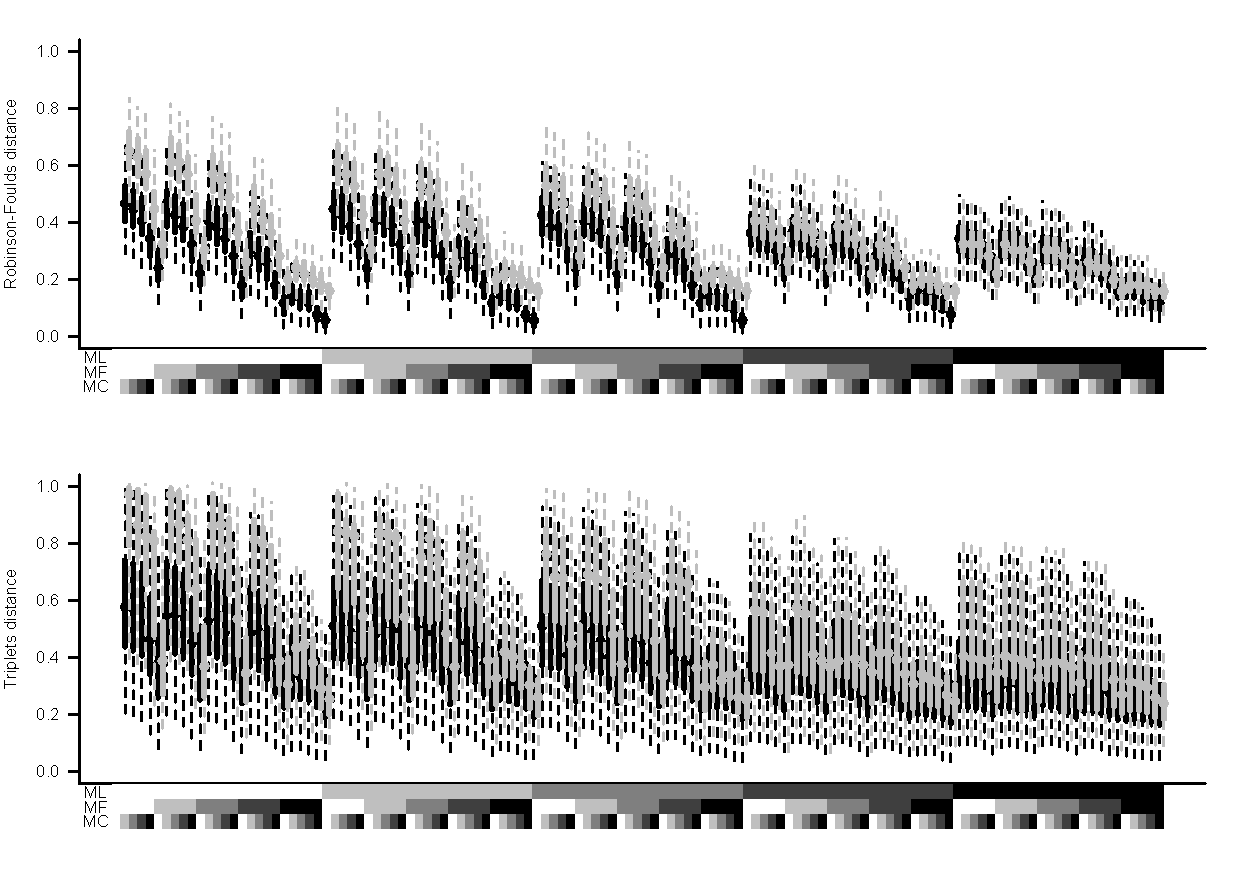
\includegraphics[width=1\textwidth]{SupplementaryMaterial/Supp_Figures/Boot+Baytre-AllParam-RF+Tr.pdf}
\caption{Trend of the effect of missing data on topological recovery on the Bootstraps and the Bayesian posterior trees distributions. The amount of missing data per parameter ($M_{L}$, $M_{F}$ and $M_{C}$) is represented along the x axis. The colour gradient from white to black represents respectively, 0\%, 10\%, 25\%, 50\% and 75\% of missing data. The topological recovery is represented on the y axis, both using Robinson-Foulds distance (upper row) and Triplets distance (lower row). Points represent the modal value of each distribution ; thick solid and thin dashed lines represents respectively the 50\% and 95\% confidence intervals or the distributions. The Bootstraps are represented in black and the Bayesian posterior trees distributions in grey.}
\label{Fig_global_BootTreesets} %Differences between all the parameters and between two methods (Boot vs treesets)
\end{figure}

\begin{figure} 
\centering
    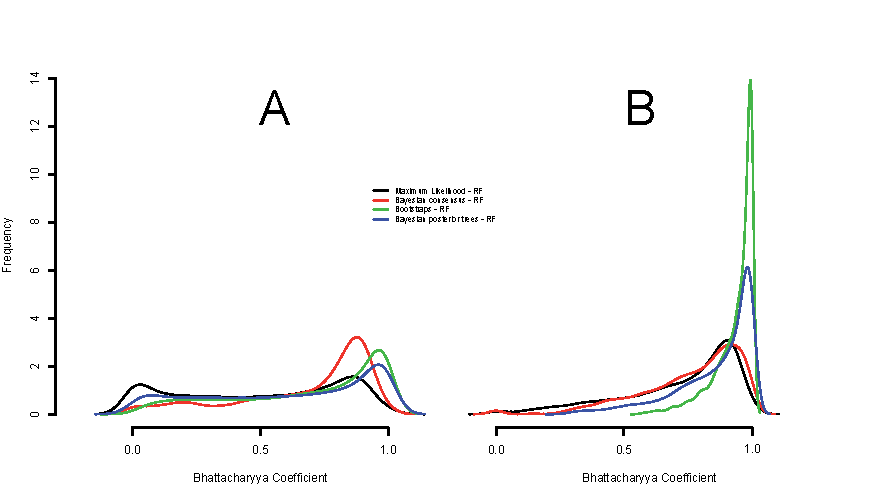
\includegraphics[width=1\textwidth]{SupplementaryMaterial/Supp_Figures/BC-AllMethods-RF+Tr.pdf}
\caption{Distribution of the Pairwise Bhattacharyya Coefficients within each method. A- Distribution of the coefficients when comparing Ronbinson-Foulds distances. B- Distribution of the coefficients when comparing Triplets distances.}
\label{Fig_Bhatt.coeff_distribution} %Differences in overlap within each method
\end{figure}

\begin{figure} 
\centering
    \includegraphics[width=1\textwidth]{SupplementaryMaterial/Supp_Figures/PairwiseComp-ML-RF+Tr.pdf}
\caption{Pairwise Bhattacharyya Coefficients within the Maximum Likelihood trees. The pairwise trees comparisons are represent on both axis. The colour gradient from white to black represents respectively, 0\%, 10\%, 25\%, 50\% and 75\% of missing data for each parameter. The matrix represents the values of pairwise Bhattacharyya Coefficients going from green (1) to red (0). A. Results for the Normalised Robinson-Foulds distance. B. Results with the for Normalised Triplets distance.}
\label{Fig_pairComp-Baytree-RF}
\end{figure} %Pairwise BC for the ML for RF+Tr. (parameters differences)

\begin{figure} 
\centering
    \includegraphics[width=1\textwidth]{SupplementaryMaterial/Supp_Figures/PairwiseComp-Boot-RF+Tr.pdf}
\caption{Pairwise Bhattacharyya Coefficients within the Bootstrap trees. The pairwise trees comparisons are represent on both axis. The colour gradient from white to black represents respectively, 0\%, 10\%, 25\%, 50\% and 75\% of missing data for each parameter. The matrix represents the values of pairwise Bhattacharyya Coefficients going from green (1) to red (0). A. Results for the Normalised Robinson-Foulds distance. B. Results with the for Normalised Triplets distance.}
\label{Fig_pairComp-Baytree-Tr}
\end{figure} %Pairwise BC for the Boot for RF+Tr. (parameters differences)

\begin{figure} 
\centering
    \includegraphics[width=1\textwidth]{SupplementaryMaterial/Supp_Figures/PairwiseComp-Baytre-RF+Tr.pdf}
\caption{Pairwise Bhattacharyya Coefficients within the Bayesian posterior distribution trees. The pairwise trees comparisons are represent on both axis. The colour gradient from white to black represents respectively, 0\%, 10\%, 25\%, 50\% and 75\% of missing data for each parameter. The matrix represents the values of pairwise Bhattacharyya Coefficients going from green (1) to red (0). A. Results for the Normalised Robinson-Foulds distance. B. Results with the for Normalised Triplets distance.}
\label{Fig_pairComp-MLbest-RF}
\end{figure} %Pairwise BC for the Baytre for RF+Tr. (parameters differences)


%Summary of metrics values for all parameters combinations
\begin{table}[ht]
\centering
\begin{tabular}{rrrrrrr}
  \hline
 & Min. & 1st Qu. & Median & Mean & 3rd Qu. & Max. \\ 
  \hline
  Maximum likelihood-RF & 0.06 & 0.26 & 0.40 & 0.41 & 0.50 & 0.95 \\ 
  Maximumlikelihood-Tr & 0.29 & 0.45 & 0.59 & 0.63 & 0.84 & 1.00 \\ 
  Bayesian consensus-RF & 0.69 & 0.71 & 0.72 & 0.76 & 0.79 & 0.96 \\ 
  Bayesian consensus-Tr & -0.28 & -0.11 & 0.17 & 0.19 & 0.37 & 0.98 \\ 
  Bootstraps-RF & 0.06 & 0.18 & 0.27 & 0.26 & 0.34 & 0.46 \\ 
  Bootstraps-Tr & 0.23 & 0.31 & 0.35 & 0.38 & 0.45 & 0.58 \\ 
  Bayesian posterior trees-RF & 0.16 & 0.22 & 0.32 & 0.34 & 0.42 & 0.65 \\ 
  Bayesian posterior trees-Tr & 0.24 & 0.35 & 0.40 & 0.50 & 0.67 & 0.98 \\ 
   \hline
   \hline
\end{tabular}
\end{table}

%Summary of metrics values for the ML parameter
\begin{table}[ht]
\centering
\begin{tabular}{rrrrrrr}
  \hline
 & Min. & 1st Qu. & Median & Mean & 3rd Qu. & Max. \\ 
  \hline
Maximum likelihood-RF & 0.44 & 0.51 & 0.63 & 0.66 & 0.78 & 0.95 \\ 
  Maximumlikelihood-Tr & 0.45 & 0.56 & 0.76 & 0.74 & 0.93 & 0.99 \\ 
  Bayesian consensus-RF & 0.71 & 0.73 & 0.80 & 0.82 & 0.88 & 0.95 \\ 
  Bayesian consensus-Tr & 0.37 & 0.46 & 0.67 & 0.67 & 0.87 & 0.96 \\ 
  Bootstraps-RF & 0.34 & 0.37 & 0.42 & 0.41 & 0.44 & 0.46 \\ 
  Bootstraps-Tr & 0.32 & 0.40 & 0.51 & 0.46 & 0.51 & 0.57 \\ 
  Bayesian posterior trees-RF & 0.33 & 0.41 & 0.52 & 0.50 & 0.60 & 0.65 \\ 
  Bayesian posterior trees-Tr & 0.41 & 0.56 & 0.76 & 0.71 & 0.84 & 0.98 \\ 
   \hline
\end{tabular}
\end{table}

%Summary of metrics values for the ML parameter
\begin{table}[ht]
\centering
\begin{tabular}{rrrrrrr}
  \hline
 & Min. & 1st Qu. & Median & Mean & 3rd Qu. & Max. \\ 
  \hline
Maximum likelihood-RF & 0.23 & 0.46 & 0.64 & 0.61 & 0.79 & 0.93 \\ 
  Maximumlikelihood-Tr & 0.65 & 0.84 & 0.95 & 0.89 & 0.99 & 1.00 \\ 
  Bayesian consensus-RF & 0.72 & 0.77 & 0.86 & 0.85 & 0.94 & 0.96 \\ 
  Bayesian consensus-Tr & -0.16 & 0.19 & 0.63 & 0.52 & 0.96 & 0.98 \\ 
  Bootstraps-RF & 0.14 & 0.30 & 0.40 & 0.35 & 0.45 & 0.46 \\ 
  Bootstraps-Tr & 0.37 & 0.49 & 0.54 & 0.51 & 0.56 & 0.57 \\ 
  Bayesian posterior trees-RF & 0.24 & 0.45 & 0.57 & 0.51 & 0.63 & 0.65 \\ 
  Bayesian posterior trees-Tr & 0.44 & 0.81 & 0.86 & 0.82 & 0.98 & 0.98 \\ 
   \hline
\end{tabular}
\end{table}

%Summary of metrics values for the MC parameter
\begin{table}[ht]
\centering
\begin{tabular}{rrrrrrr}
  \hline
 & Min. & 1st Qu. & Median & Mean & 3rd Qu. & Max. \\ 
  \hline
Maximum likelihood-RF & 0.40 & 0.50 & 0.64 & 0.65 & 0.79 & 0.94 \\ 
  Maximumlikelihood-Tr & 0.70 & 0.84 & 0.93 & 0.89 & 0.99 & 1.00 \\ 
  Bayesian consensus-RF & 0.76 & 0.79 & 0.86 & 0.86 & 0.92 & 0.96 \\ 
  Bayesian consensus-Tr & 0.05 & 0.16 & 0.53 & 0.50 & 0.87 & 0.92 \\ 
  Bootstraps-RF & 0.25 & 0.34 & 0.42 & 0.38 & 0.45 & 0.46 \\ 
  Bootstraps-Tr & 0.38 & 0.47 & 0.55 & 0.51 & 0.57 & 0.58 \\ 
  Bayesian posterior trees-RF & 0.32 & 0.44 & 0.58 & 0.52 & 0.62 & 0.65 \\ 
  Bayesian posterior trees-Tr & 0.39 & 0.78 & 0.82 & 0.79 & 0.98 & 0.98 \\ 
   \hline
\end{tabular}
\end{table}


%Summary of the BC between pairs of methods for the ML parameter
\begin{table}[ht]
\centering
\begin{tabular}{rrrrrrr}
  \hline
 & Min. & 1st Qu. & Median & Mean & 3rd Qu. & Max. \\ 
  \hline
Maximum.likelihood.vs..Bayesian.consensus...RF & 0.30 & 0.31 & 0.69 & 0.61 & 0.77 & 1.00 \\ 
  Maximum.likelihood.vs..Bayesian.consensus...Tr & 0.79 & 0.81 & 0.84 & 0.86 & 0.85 & 1.00 \\ 
  Maximum.likelihood.vs..Bootstraps...RF & 0.03 & 0.22 & 0.29 & 0.36 & 0.54 & 0.69 \\ 
  Maximum.likelihood.vs..Bootstraps...Tr & 0.08 & 0.42 & 0.53 & 0.51 & 0.74 & 0.78 \\ 
  Maximum.likelihood.vs..Bayesian.posterior.trees...RF & 0.02 & 0.49 & 0.61 & 0.51 & 0.67 & 0.74 \\ 
  Maximum.likelihood.vs..Bayesian.posterior.trees...Tr & 0.21 & 0.61 & 0.70 & 0.63 & 0.81 & 0.81 \\ 
  Bayesian.consensus.vs..Bootstraps...RF & 0.01 & 0.02 & 0.02 & 0.02 & 0.03 & 0.04 \\ 
  Bayesian.consensus.vs..Bootstraps...Tr & 0.08 & 0.69 & 0.78 & 0.64 & 0.79 & 0.84 \\ 
  Bayesian.consensus.vs..Bayesian.posterior.trees...RF & 0.01 & 0.02 & 0.02 & 0.04 & 0.08 & 0.09 \\ 
  Bayesian.consensus.vs..Bayesian.posterior.trees...Tr & 0.21 & 0.74 & 0.75 & 0.68 & 0.84 & 0.87 \\ 
  Boostraps.vs..Bayesian.posterior.trees...RF & 0.69 & 0.75 & 0.85 & 0.85 & 0.95 & 1.00 \\ 
  Boostraps.vs..Bayesian.posterior.trees...Tr & 0.91 & 0.92 & 0.96 & 0.95 & 0.97 & 0.98 \\ 
   \hline
\end{tabular}
\end{table}

%Summary of the BC between pairs of methods for the MF parameter
\begin{table}[ht]
\centering
\begin{tabular}{rrrrrrr}
  \hline
 & Min. & 1st Qu. & Median & Mean & 3rd Qu. & Max. \\ 
  \hline
Maximum.likelihood.vs..Bayesian.consensus...RF & 0.00 & 0.25 & 0.48 & 0.50 & 0.76 & 1.00 \\ 
  Maximum.likelihood.vs..Bayesian.consensus...Tr & 0.38 & 0.69 & 0.75 & 0.72 & 0.80 & 1.00 \\ 
  Maximum.likelihood.vs..Bootstraps...RF & 0.03 & 0.18 & 0.32 & 0.36 & 0.47 & 0.77 \\ 
  Maximum.likelihood.vs..Bootstraps...Tr & 0.08 & 0.34 & 0.40 & 0.38 & 0.53 & 0.55 \\ 
  Maximum.likelihood.vs..Bayesian.posterior.trees...RF & 0.02 & 0.47 & 0.71 & 0.60 & 0.86 & 0.94 \\ 
  Maximum.likelihood.vs..Bayesian.posterior.trees...Tr & 0.21 & 0.54 & 0.62 & 0.56 & 0.64 & 0.80 \\ 
  Bayesian.consensus.vs..Bootstraps...RF & 0.00 & 0.00 & 0.01 & 0.01 & 0.01 & 0.03 \\ 
  Bayesian.consensus.vs..Bootstraps...Tr & 0.08 & 0.38 & 0.54 & 0.49 & 0.70 & 0.75 \\ 
  Bayesian.consensus.vs..Bayesian.posterior.trees...RF & 0.00 & 0.02 & 0.02 & 0.02 & 0.04 & 0.04 \\ 
  Bayesian.consensus.vs..Bayesian.posterior.trees...Tr & 0.21 & 0.29 & 0.66 & 0.54 & 0.72 & 0.82 \\ 
  Boostraps.vs..Bayesian.posterior.trees...RF & 0.69 & 0.69 & 0.72 & 0.71 & 0.72 & 0.72 \\ 
  Boostraps.vs..Bayesian.posterior.trees...Tr & 0.91 & 0.91 & 0.91 & 0.93 & 0.92 & 0.98 \\ 
   \hline
\end{tabular}
\end{table}

%Summary of the BC between pairs of methods for the MC parameter
\begin{table}[ht]
\centering
\begin{tabular}{rrrrrrr}
  \hline
 & Min. & 1st Qu. & Median & Mean & 3rd Qu. & Max. \\ 
  \hline
Maximum.likelihood.vs..Bayesian.consensus...RF & 0.03 & 0.32 & 0.66 & 0.55 & 0.75 & 1.00 \\ 
  Maximum.likelihood.vs..Bayesian.consensus...Tr & 0.51 & 0.69 & 0.80 & 0.76 & 0.80 & 1.00 \\ 
  Maximum.likelihood.vs..Bootstraps...RF & 0.03 & 0.17 & 0.21 & 0.31 & 0.46 & 0.68 \\ 
  Maximum.likelihood.vs..Bootstraps...Tr & 0.08 & 0.31 & 0.39 & 0.39 & 0.56 & 0.61 \\ 
  Maximum.likelihood.vs..Bayesian.posterior.trees...RF & 0.02 & 0.44 & 0.47 & 0.52 & 0.78 & 0.90 \\ 
  Maximum.likelihood.vs..Bayesian.posterior.trees...Tr & 0.21 & 0.52 & 0.59 & 0.55 & 0.66 & 0.77 \\ 
  Bayesian.consensus.vs..Bootstraps...RF & 0.00 & 0.01 & 0.01 & 0.02 & 0.02 & 0.03 \\ 
  Bayesian.consensus.vs..Bootstraps...Tr & 0.08 & 0.47 & 0.62 & 0.51 & 0.66 & 0.73 \\ 
  Bayesian.consensus.vs..Bayesian.posterior.trees...RF & 0.00 & 0.02 & 0.04 & 0.04 & 0.05 & 0.06 \\ 
  Bayesian.consensus.vs..Bayesian.posterior.trees...Tr & 0.21 & 0.45 & 0.64 & 0.57 & 0.74 & 0.79 \\ 
  Boostraps.vs..Bayesian.posterior.trees...RF & 0.69 & 0.73 & 0.73 & 0.76 & 0.81 & 0.86 \\ 
  Boostraps.vs..Bayesian.posterior.trees...Tr & 0.91 & 0.92 & 0.93 & 0.94 & 0.96 & 0.99 \\ 
   \hline
\end{tabular}
\end{table}
  \label{Supp_results}

%END
\end{document}
    \label{SupplementaryMaterial}

%END
\end{document}